For improving the object detection neural-network we implemented some data distorsion methons, which simulate wheater conditions:
\begin{itemize}
    \item \emph{light-rain:} A little blur to the image and random generated lines
    \item \emph{normal-rain:} Same as light-rain, but more lines
    \item \emph{snow:} Change the color of some part of picture to white to simulate snow.
    \item \emph{sun:} Increase brigthness for simulating a sunny day
\end{itemize}

These methods where found in this link: \url{https://www.freecodecamp.org/news/image-augmentation-make-it-rain-make-it-snow-how-to-modify-a-photo-with-machine-learning-163c0cb3843f/}

After we find all the rectangles in the original imagages we distored the image and give it to the neural network with the found rects
for learning resource. This way it could train itself for more drastic enviromental conditions.
\begin{figure}[!htb]
    \centering
    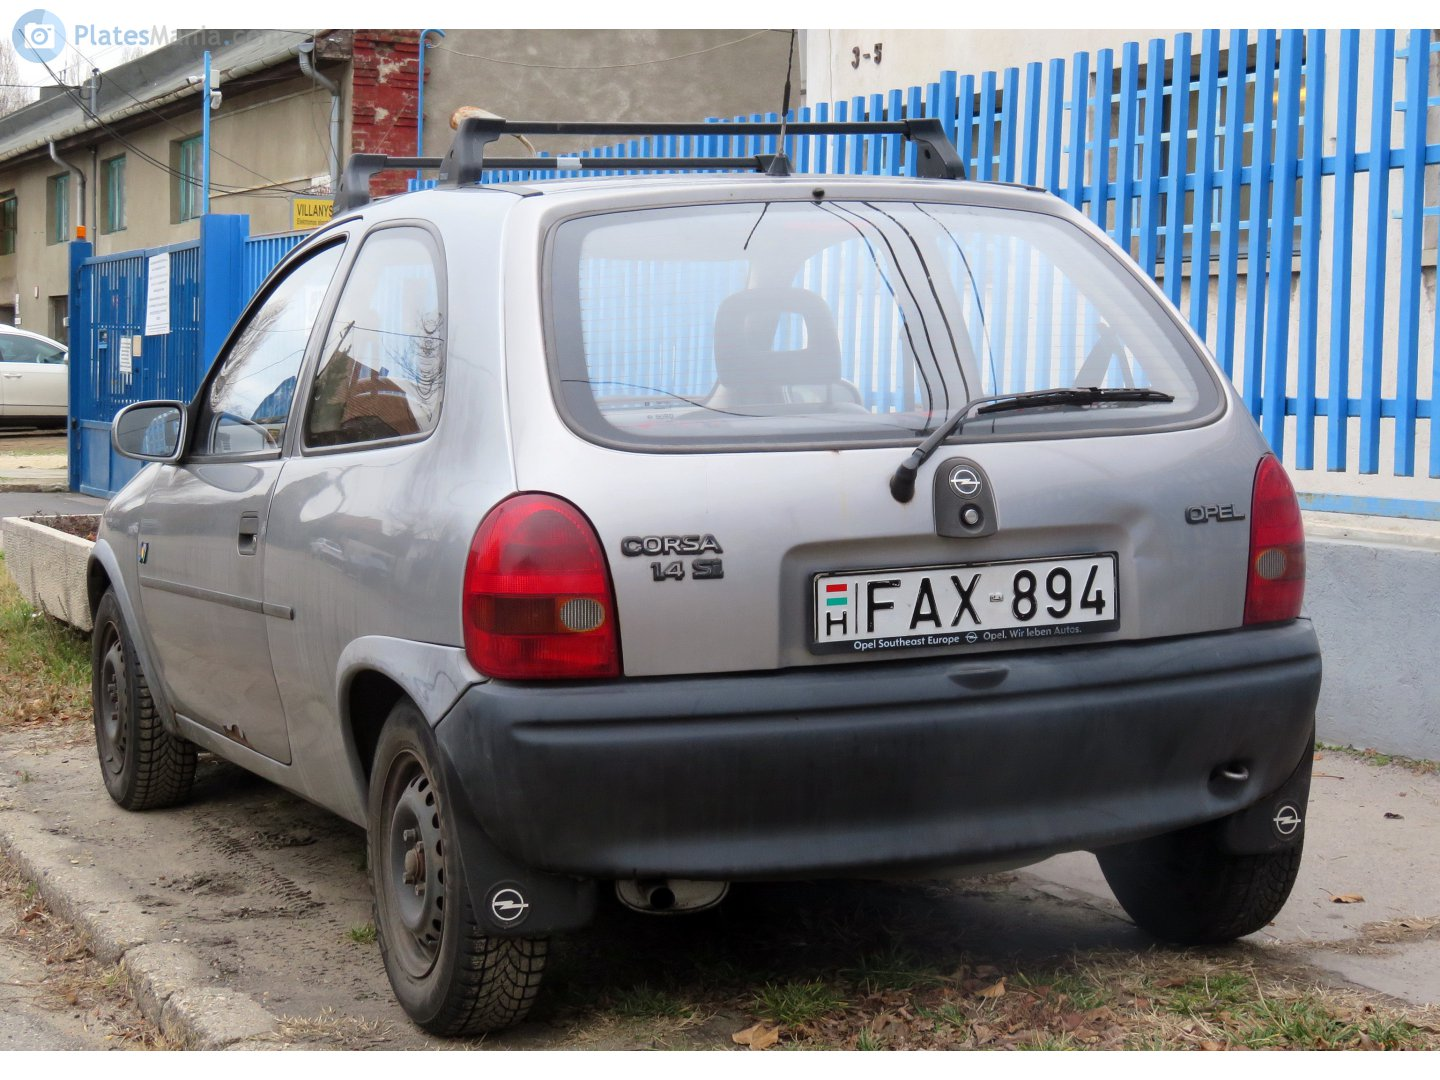
\includegraphics[width=0.5\textwidth]{figures/original.jpg}
    \caption{Original Image}
    \label{fig:wheater-original}
\end{figure}
\begin{figure}[!htb]
    \begin{subfigure}[b]{.45\textwidth}
        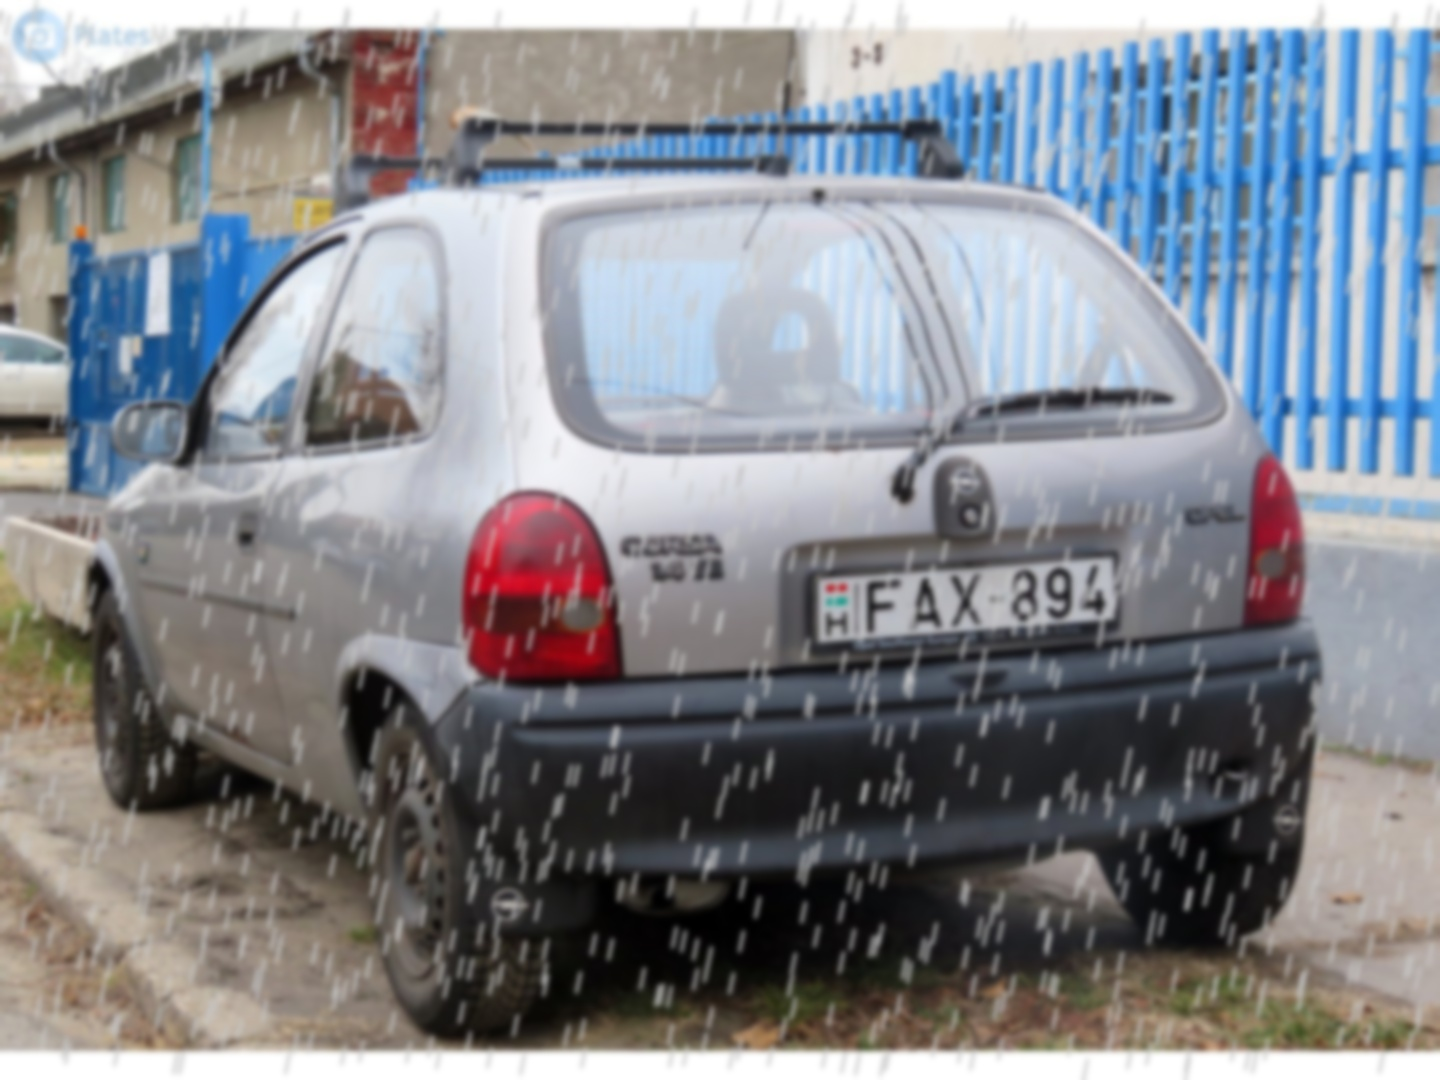
\includegraphics[width=\textwidth]{figures/lightrain.jpg}
    \end{subfigure}
    \hfill
    \begin{subfigure}[b]{.45\textwidth}
        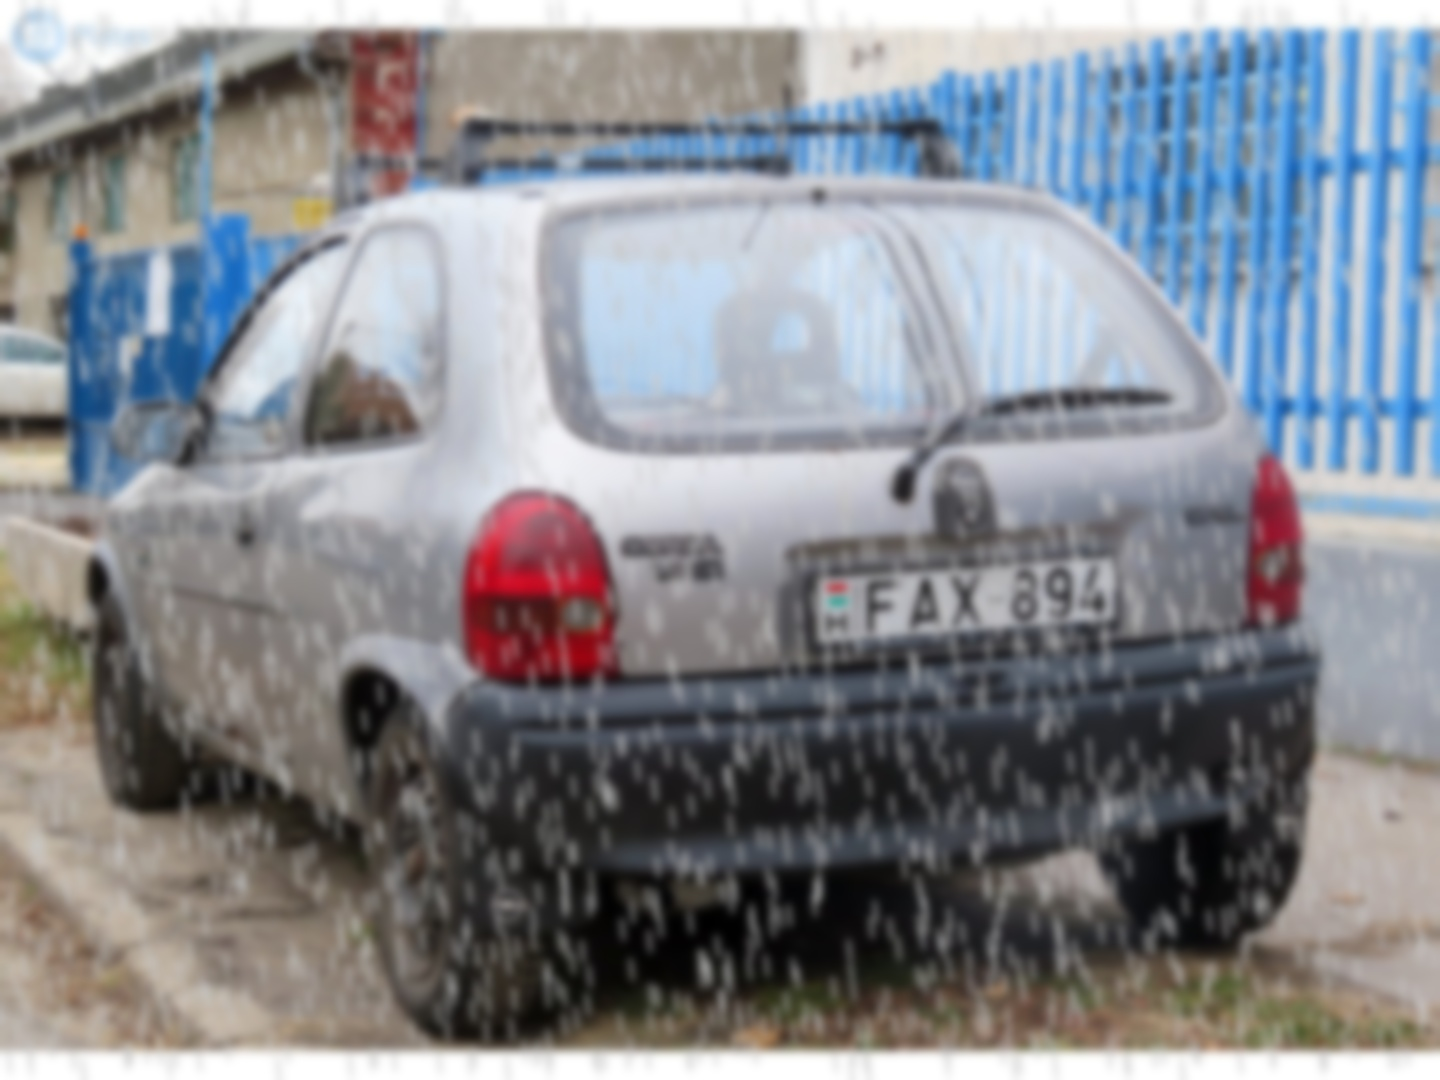
\includegraphics[width=\textwidth]{figures/rain.jpg}
    \end{subfigure}
    \hfill
    \caption{Two types of rain}
    \label{fig:wheater-raines}
\end{figure}
\begin{figure}[!htb]
    \begin{subfigure}[b]{.45\textwidth}
        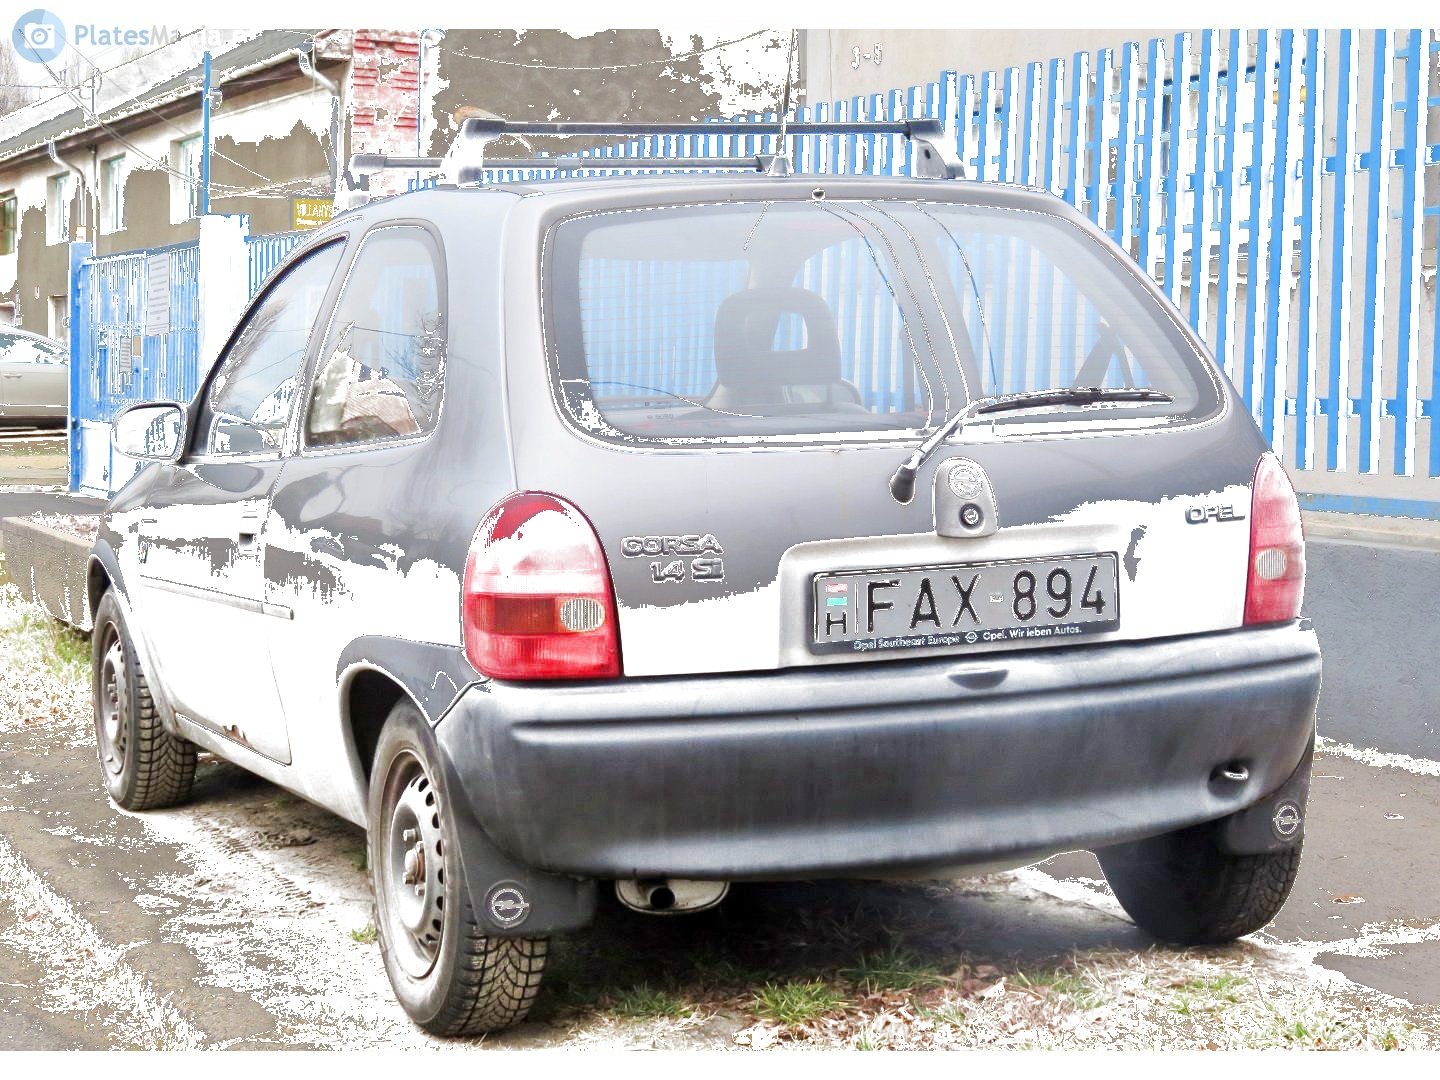
\includegraphics[width=\textwidth]{figures/snow.jpg}
    \end{subfigure}
    \hfill
    \begin{subfigure}[b]{.45\textwidth}
        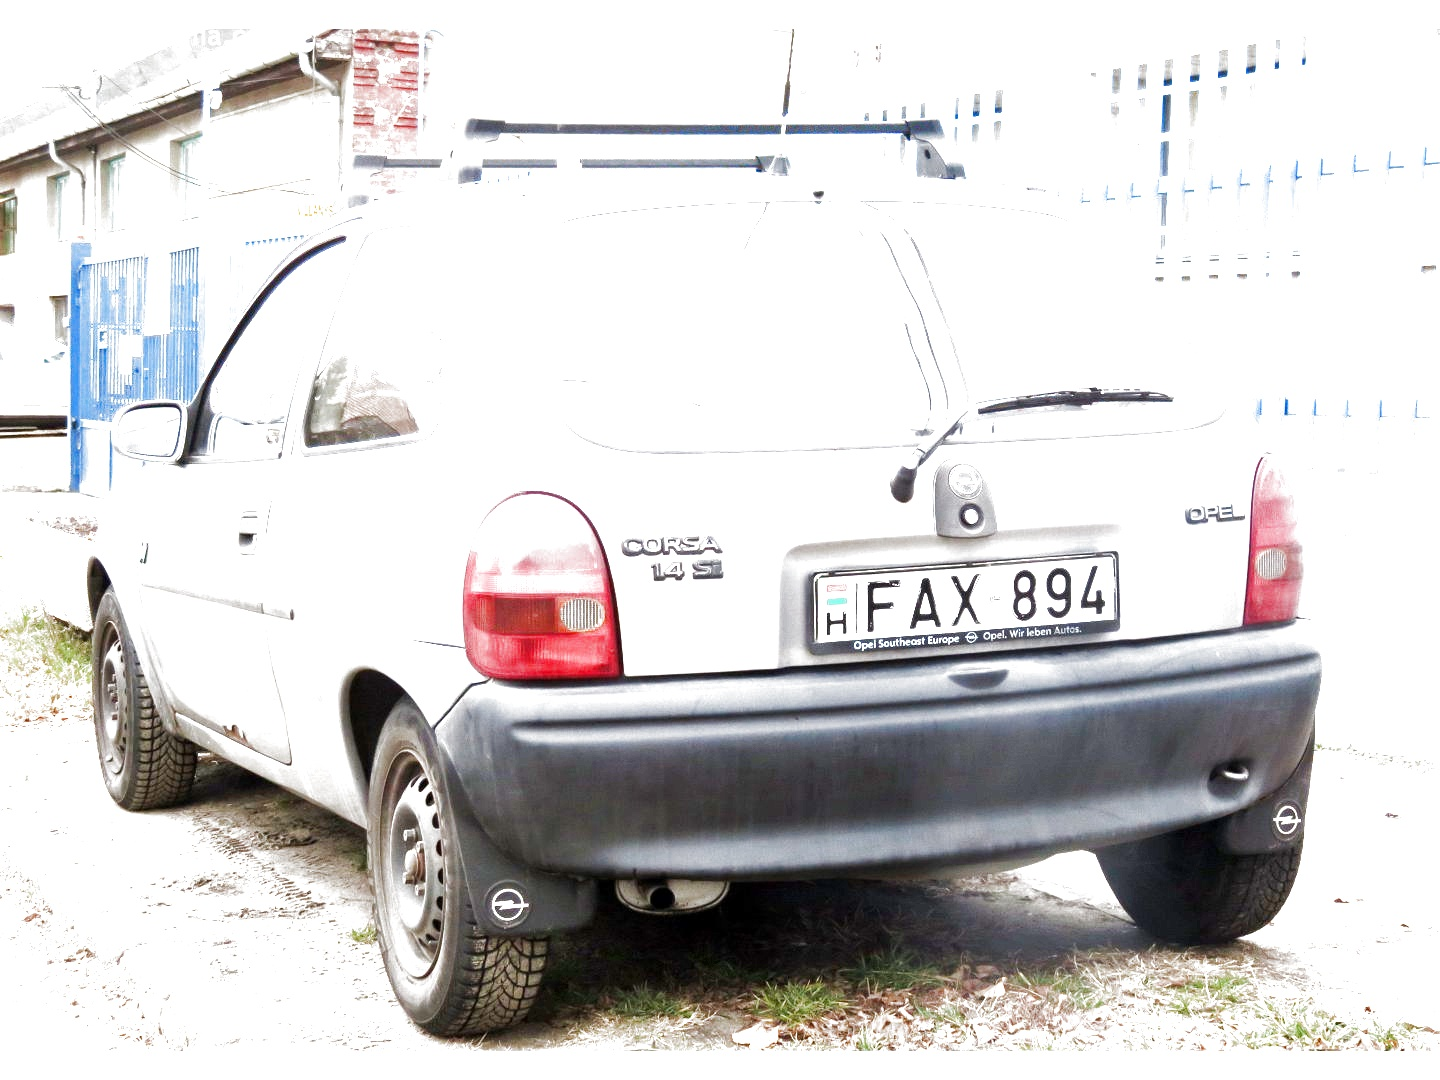
\includegraphics[width=\textwidth]{figures/sunny.jpg}
    \end{subfigure}
    \hfill
    \caption{Snow and Sun filter}
    \label{fig:wheater-snow-sun}
\end{figure}
